\documentclass[12pt]{article}  % do not change this line!
\author{Mostafa Rizk, Julian Garcia, Aldeida Aleti, Giuseppe Cuccu}
\usepackage{booktabs}
\usepackage{amsmath}
\usepackage[colorinlistoftodos,prependcaption,textsize=tiny]{todonotes}


\begin{document}

\title{Effective Evolution of Task Specialisation in Multi-Robot Teams}  
\maketitle

%%%%%%%%%%%%%%%%%%%%%%%%%%%%%%%%%%%%%%%%%%%%%%%%%%%%%%%%%%%%%%%%%%%%%%%%%%%%%%%%%%%%%%%%%%%%%%%%%%%%%%%%%
%% start of main body of paper

\section{Introduction}

Aim is to evolve a multi-agent team that solves a task in a partitioned way. 
Also to understand the qualities of the fitness landscape in such a task for each of four evolutionary configurations. 

\section{Background}

Khamis et al review multi-robot task allocation. Evolution is one approach. Less manual programming. In theory, don’t need to analyse each new task.
Pini et al manually programmed agents that alternate between generalist and specialist strategy.
Ferrante et al \cite{ferrante:PLOS_CB:2015} evolved specialisation 
Waibel et al studied 4 evolutionary configurations \cite{waibel:Transactions:2009}

\section{Experimental Methods}

\subsection{The Foraging Task}

We use a foraging task as the testbed for the evolution of specialisation.
The task is modelled off the foraging behaviour of the Atta Leafcutter ant, as in Ferrante et al \cite{ferrante:PLOS_CB:2015} and Pini et al \cite{pini:Swarm_Intelligence:2011; pini:ICSI:2012}.
In nature, the ants cut leaves from a tree and take them to their nest. 
Sometimes the ants partition the task. 
When they do so, some ants are droppers, who cut leaves and let them fall, while other ants are collectors who collect fallen leaves from the base of the tree and take them to the nest.
This partitioned approach is advantageous because gravity transports leaves faster than ants can.
Rather than every ant climbing up the tree, cutting a leaf and bringing it to the nest, when they partition the ants are able to transport more leaves in the same time-span while consuming less energy.
We model this scenario similarly to Ferrante et al \cite{ferrante:PLOS_CB:2015}, with a slope in place of the tree trunk.
Much like the ants, agents transport resources from the source to the nest.
An agent on a team can use a generalist strategy where it acts individually, going up and down the slope to retrieve resources.
An agent can also use a specialist strategy. 
As a specialist it can either be a dropper, going up the slope once and dropping things from the nest, or it can be a collector and gather the resources that accumulate at the base of the slope, called the cache.
Much like real robots that deplete their battery and ants that deplete their energy stores, there is a cost to moving and it is compounded when going up the slope. 
Teams that use complementary specialist strategies pay a smaller energy cost as well as time cost, since resources slide down faster than they can be carried. 
Preliminary analysis with hand-coded agents verifies that specialist teams gain higher overall reward than generalist teams.\\

More formally, you have a team of $n_{agents}$ agents. 
They are placed in a rectangular arena that is $l$ tiles long and $w$ tiles wide, illustrated in Figure \ref{fig:arena}. 
The arena is divided into four sections $l= l_{nest} + l_{cache} + l_{slope} + l_{source}$.
Each episode is composed of a number of finite time-steps $t=0, .... T$. 
Since 3D physics is computationally expensive we use a 2D environment to expedite our experiments as the focus of our research is on the evolutionary process and team dynamics rather than the robotic element.
We also use a discrete scenario, as opposed to a continuous one for further simplicity.
To simulate the presence of gravity, resources move when on the slope, at a speed greater than the agents are capable of.
The high sliding speed creates evolutionary pressure for the team to specialise.
Agents travel at speed $s_{agent}$ and resources slide when placed on the slope with a speed of $s_{resource}$ 
Additionally agents pay costs for moving.
This simulates the presence of a battery, with energy expenditure varying depending on where the agent is moving.
There is a base cost to moving $c$ paid by the agent for moving in any direction.
The base cost is multiplied by different factors for moving up the slope ($f_{up}$) down the slope ($f_{down}$) and moving while carrying a resource ($f_{carry}$). 
An agent moving sideways on the slope pays the same cost as one moving on a non-slope area in any direction.
An agent moving one tile up the slope at time step $t=0$ while carrying a resource, for example, pays a cost of $C_{0} = f_{up} \cdot f_{carry} \cdot c$ .
There are $n_{resources}$ resources at the source, initially.
Every time a resource is removed from the source, another one appears at the source so there are always at least $n_{resources}$.
Each resource retrieved provides all team members a reward of $R$.
The values we chose for these parameters can be found in the appendix\\

Fitness can be calculated for the team or for an individual depending on the level of selection.
When calculating fitness for a team of agents, the fitness function is as follows:\\ 
\\
$F = \sum_{t=1}^{T} \sum_{i}^{n_{agents}} (R_{ti} - C_{ti}) $\\
\\
That is, for each agent, at each time step, we calculate the reward it received at that time step (whether from retrieving a resource itself or from another agent retrieving a resource) and we subtract the cost it individually paid at that time step. 
We then take the summation of this calculation for all agents over all time steps in the simulation.
The reward and cost for an agent $i$ at time step $t$ can be computed as shown here:\\
\\
$
R_{ti} = R \cdot r_{t}
$\\
\\
where $r_t$ is the total number of resources retrieved by all agents at time $t$
\\
\\
\\
$
C_{ti} = \left\{
        \begin{array}{ll}
            c & \quad not on slope or moved sideways on slope\\
            c \cdot f_{up} & \quad up slope\\
            c \cdot f_{down} & \quad down slope\\
            c \cdot f_{carry} & \quad not on slope or moved sideways on slope while carrying\\
            c \cdot f_{carry} \cdot f_{up} & \quad up slope while carrying \\
            c \cdot f_{carry} \cdot f_{down} & \quad down slope while carrying\\
        \end{array}
    \right.
$
\\
\\
When calculating fitness for an individual agent, the fitness function is as follows:\\
\\
$F = \sum_{t=1}^{T} (R_{ti} - C_{ti}) $
\\
\\
Example: Agent 1 incurs -200 retrieving resource. 
Agent 2 incurs -100 wandering around cache. 
Agent 1 score= 1000 - 200. 
Agent 2 score = 1000 - 100.
Team selection: team score = agent 1 score + agent 2 score = 800 + 900 = 1700
Individual selection: agent 1 score = 800, agent 2 score = 900. 
In team selection, team is compared to other teams. 
In individual selection, highest scoring individual is selected. 

\begin{figure}
	\centering
	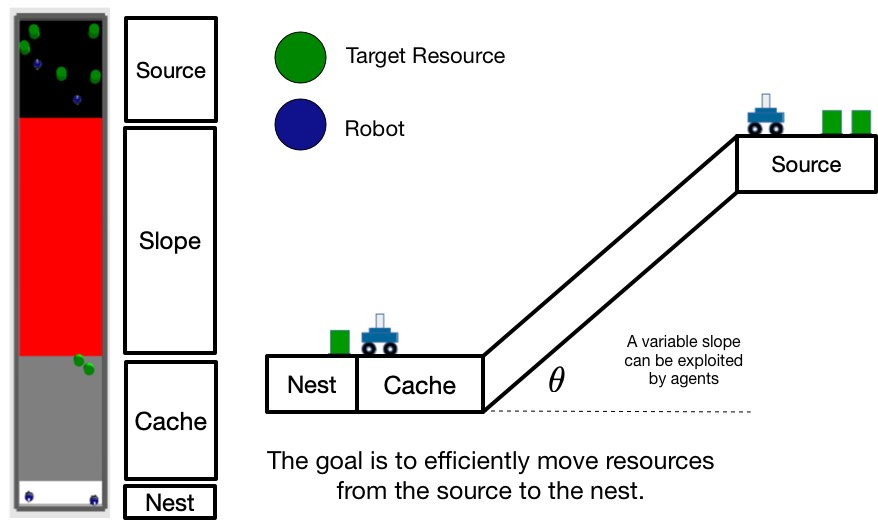
\includegraphics[width=\textwidth]{arena.jpg}
	\caption{Arena Layout}
	\label{fig:arena}
\end{figure}

\subsection{Observations and Actions}

Agents have a sensing range that indicates how many tiles around them they can observe. 
A sensing range of 0 means an agent can just observe the current tile it is on. 
A range of 1 means it can observe a square centred  on its location that extends 1 tile in each direction (9 tiles total including current tile). 
A range of 2 means it can observe a square extending 2 tiles in each direction (25 tiles total). 
And so on.
We assume our agent represents a robot with only local sensing capabilities and use a sensing range of 1, which has the added benefit of reducing computation.
For each tile in its sensing range, an agent observes a onehotencoded 4-bit vector. 
The values it reads denote the following: Blank= 1000, Agent = 0100, Resource = 0010, Wall = 0001.
Tiles are read row by row from top left to bottom right. 
The next part of an agent's observation is a 4-bit vector denoting which part of the arena it is on, similar to a real robot with a ground sensor that can detect the unique colour of each area.
The values of this vector can be as follows: Nest = 1000, Cache = 0100, Slope = 0010, Source = 0001
The final part of an agent's observation is 1-bit for resource possession. 
The values can be as follows: Has resource = 1, Doesn’t have resource = 0
The total length of the observation vector is 9x4 + 4 + 1= 41 bits.\\

An agent can perform 6 possible actions, represented by the following values: Forward = 0, Backward = 1, Left = 2, Right = 3, Pick-up = 4, Drop = 5.
We use a recurrent neural network to choose actions based on the observed state.
Since many of the positions in the environment will produce the same observation, a recurrent neural network gives the agent to have a simple form of memory, preventing it from getting "stuck" in infinite state transition loops.
The network has 41 inputs, 1 bias input and 6 recurrent inputs (one for each of the 6 outputs). 
There is no hidden layer, just a 6-neuron output layer. 
This makes for a total of (41+1+6)x6 = 288 weights. 
The output layer uses a linear activation function.

\subsection{Evolutionary Algorithm}

We use the CMA-ES (CMA) algorithm. 
While a traditional GA maintains a population of solutions, CMA-ES maintains a probability distribution with a mean and sigma, sampling any number of individuals from that distribution. 
The fitness of those individuals is used to update the mean and sigma, while keeping track of the best solution so far. 
CMA parameters are set according to the default values in this implementation, however we change the following:
Maxiter = 5000 generations, pop size = 40 (80 for Het-Ind and Hom-Ind), tolx = 1e-3, tolfunhist = 2e2
Population size is different because the number of teams is held constant (40 teams). 
If we're using team level selection, the genome contains all team members. 
When the algorithm selects a genome, in this case, it is selecting an entire team.
If we're using individual level selection, the genome contains a single individual. 
When the algorithm selects a genome in this case, it is selecting a single member of the team. 
When using individual selection with teams of two agents, there are two genomes per team thus 80 genomes in the population.
Tolx is a termination criterion that terminates the algorithm's current run if the mean, x, changes by less than tolx. 
This ensures that the algorithm stops if the genomes aren’t being changed by much. 
Tolfunhist is a termination criterion that terminates the algorithm's run if the best fitnesses over several generations haven't changed by much. 
A history variable in the code stores the best fitness at a generation. 
The difference between the minimum and maximum values in the history is calculated. 
If the difference is less than tolfunhist, the algorithm terminates. 
Essentially, if the best fitness varies by less than 2000 over 9 generations, the algorithm terminates.\\
 
We bootstrap evolution using the random weight guessing algorithm. 
Running evolution on its own we find that the algorithm suffers from a flat fitness landscape.
Bootstrapping allows us to start evolution from a genome that is slightly better than random behaviour to bypass the flat fitness issue.
In RWG, we do 10,000 runs of the environment with different seeds with 5 trials for each seed. 
Agent and resource positions are randomised in each trial.
The best genome found at the end of RWG is returned and used as the mean for CMA-ES.

\subsection{Team Composition and Level of Selection}

During the evolutionary process, it is possible to have four different combinations of team composition and level of selection that impact evolution.
A team can be either homogeneous, with all agents having the same genome, or it can be heterogeneous, with agents having different genomes.
In our case, a heterogeneous team has two different genomes, with half the team having one genome and the other half of the team having the other.
During evolution, team selection can be used, where an entire team of agents can be selected based on the collective fitness of all agents on the team.
Individual selection can also be used, where each agent on the team has its fitness considered separately.
In the latter case, an individual agent with a high reward and low cost can be selected while its team-mates are discarded. 
The four combinations are thus: heterogeneous team with team selection (Het-Team), homogeneous team with team selection (Hom-Team), heterogeneous team with individual selection (Het-Ind) and homogeneous team with individual selection (Hom-Ind).\\



\subsubsection{Homogeneous Team with Team Selection}

A genome is the weights for one neural network (288 weights) and all agents on a team load that genome into their neural network.
There are 40 teams so 40 genomes are created. 
All members of the team share the reward and cost and a fitness value is returned for the team.
40 fitness values are returned for the whole generation. 
The genome used by the best performing team is selected.\\

\subsubsection{Heterogeneous Team with Individual Selection}

A genome is the weights for one neural network (288 weights).
Each agent on the team receives its own genome.
There are 40 teams with two members per team so 80 genomes are created.  
For every two genomes, half the robots on the team get the first genome and half the robots on the team get the second. 
Team members are evaluated separately. 
They share the reward but bear costs separately. 
A fitness value is returned for each team member so 80 fitness values are returned for the whole generation. 
The genome used by the best performing individual on any team is selected. \\



\section{Experiments}

\subsection{Evolving Specialisation}
Using hardcoded controllers for agents, we observe the rewards illustrated in Figure \ref{fig:hardcoded}. We see that a team with two generalists performs well but one with a dropper and collector cooperating performs better. We run evolution using 30 different random seeds and find that most teams perform very poorly, with some outliers achieving higher scores (Figure \ref{fig:evolved}) but low specialisation (\ref{fig:evolved_spec}). \\

\begin{figure}
	\centering
	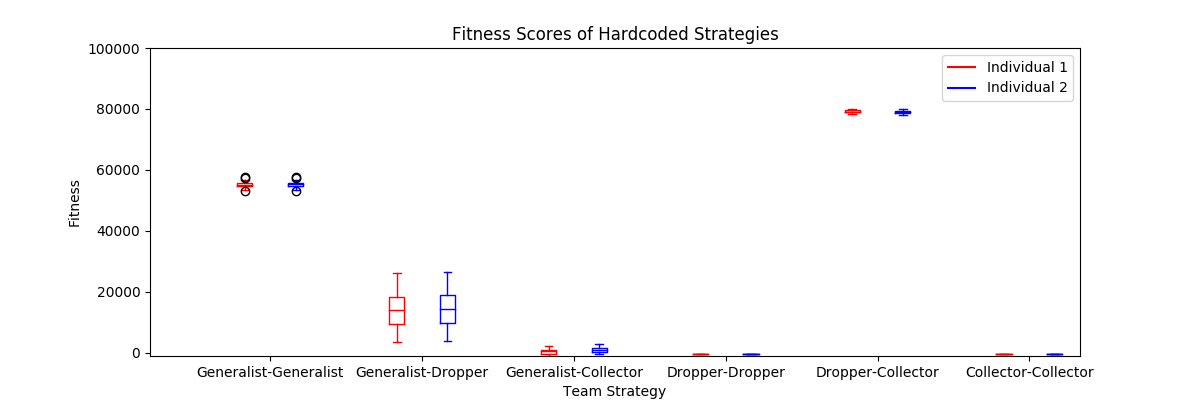
\includegraphics[width=\textwidth]{hardcoded_fitness.png}
	\caption{Fitness of Hardcoded Strategies}
	\label{fig:hardcoded}
\end{figure}

\begin{figure}
	\centering
	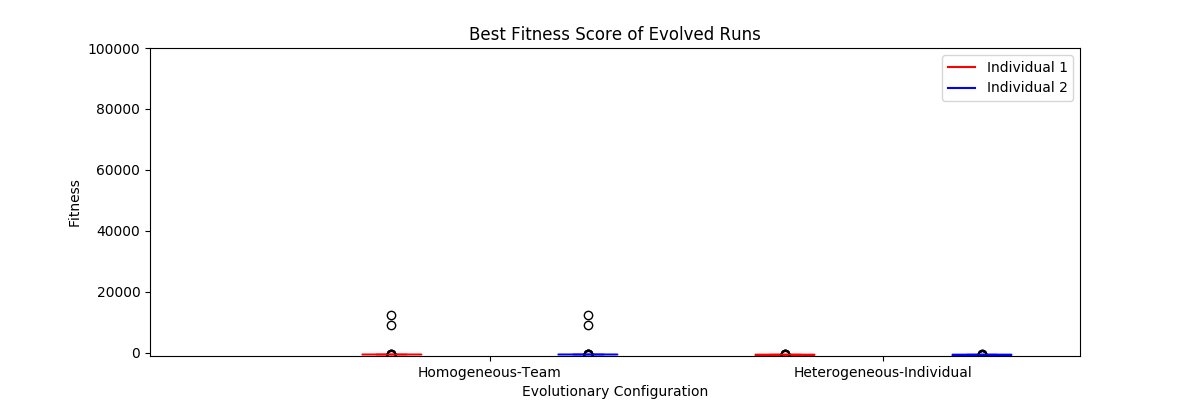
\includegraphics[width=\textwidth]{evolution_fitness.png}
	\caption{Fitness of Evolved Strategies}
	\label{fig:evolved}
\end{figure}

\begin{figure}
	\centering
	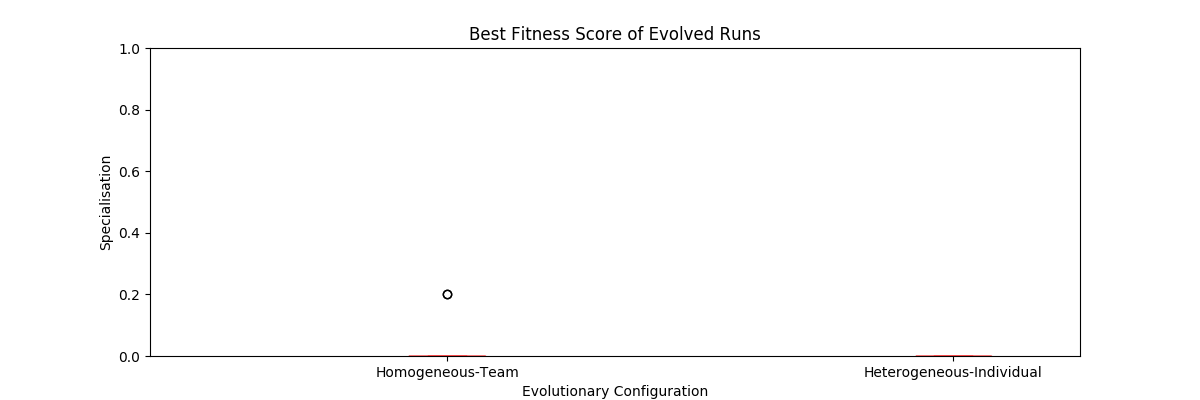
\includegraphics[width=\textwidth]{evolution_specialisation.png}
	\caption{Specialisation of Evolved Strategies}
	\label{fig:evolved_spec}
\end{figure}





\subsection{Analysing the Fitness Landscape}
We run bootstrapping and evolution for 50 seeds for each of the four configurations. A total of 200 experiments. 
We sample the generated genomes and their logged fitnesses throughout the process and then use flacco to model the fitness landscape based on this data.\\

[Visualisation of fitness landscape for each configuration]

\subsection{Modified Evolution}

We modify the evolutionary algorithm based on the results of the landscape.

\section{Discussion}

\subsection{Modelling Foraging as a Stag Hunt Game}

The foraging scenario we use here can be modelled as a stag hunt game.
In a stag hunt game with two agents, each agent can adopt either a generalist or a specialist strategy. 
If both adopt the generalist strategy it is a stable equilibrium but has lower payoff than if both adopt a specialist strategy.
However, if one agent adopts a specialist strategy while the other is generalist, it has lower payoff than if it too was a generalist.
This is a slightly more complex variant of the stag hunt game since the agents must not simply be specialists, but the right ratio of droppers and collectors. This is illustrated in Table \ref{tab:payoffs}\\

\begin{table}
\begin{center}
\begin{tabular}{ |c|c|c|c| } 
 \hline
  & Generalist & Dropper & Collector  \\ 
 \hline
 \hline
 Generalist & 54,035 + 54,045  & 13,829 + 14,146 & 2232 + 2700 \\ 
 \hline
 Dropper &  & -448 + -392 & 78,958 + 78,740 \\ 
 \hline
 Collector &  &  & -500 + -500 \\ 
 \hline
 \end{tabular}
\caption{\label{tab:payoffs}Payoffs of Strategies}
\end{center}
\end{table}
\todo{Fix code so that Dropper-Dropper etc work correctly together}


\section{Conclusion}

TODO

\bibliographystyle{plain}
\bibliography{references.bib}

\section{Appendix}

\subsection{Parameters}

\begin{center}
\begin{tabular}{ |c|c| } 
 \hline
 Parameter & Value  \\ 
 \hline
 \hline
 $l$ & 8  \\ 
 \hline
 $w$ & 4  \\ 
 \hline
 $n_{agents}$ & 2  \\ 
 \hline
 $n_{resources}$ & 3  \\ 
 \hline
 $l_{nest}$ & 1  \\ 
 \hline
 $l_{cache}$ & 2  \\ 
 \hline
 $l_{slope}$ & 4  \\ 
 \hline
 $l_{source}$ & 1  \\ 
 \hline
 $s_{agent}$ & 1  \\ 
 \hline
 $s_{resource}$ & 4  \\ 
 \hline
 $c$ & 1  \\ 
 \hline
 $f_{up}$ & 3  \\ 
 \hline
 $f_{down}$ & 0.2  \\ 
 \hline
 $f_{carry}$ & 2  \\ 
 \hline
 $R$ & 1000  \\ 
 \hline
 $T$ & 500  \\ 
 \hline
 
\end{tabular}
\end{center}

\subsubsection{Selecting Parameter Values}

$l$- If the arena is too short, resources sliding down the slope do not provide a significant time advantage over an agent carrying them. If the arena is too long, random agents produced at the beginning of evolution are less likely to travel up the slope long enough to pick up a resource and then travel down the slope long enough to return the resource. Longer simulations would be necessary, increasing overall computation time. \\

$n_{agents}$- This number must be even so that on heterogeneous teams, there is an equal number of agents having each of the two genomes. Preliminary experiments were done that showed that a larger number of agents (given the chosen arena width) results in deadlocks that prevent the agents from moving for several time-steps or the entire simulation.\\

$n_{resources}$- \\

\subsection{Hardcoded Strategies}
\todo{Pseudocode for hardcoded strategies}

\end{document}